In this section, we discuss a representative running examples with
challenges of analyzing the symbolic
\emph{reachability-bound} on
every control location and illustrate our key novelties, \emph{path reachability-bound} and the \emph{loop reachability-bound}.
This example is adopted from the example in~\cite{GulwaniZ10}, which
is a skeleton code from the .Net base-class library.

% \paragraph{Challenges.}
\begin{example}
  [The Running Example with Two Paths Loop and Nested Loop in One Path]
  \label{ex:relatedNestedWhileOdd_abscfg}
    { \small
  \begin{figure}
  \centering
  \begin{subfigure}{.4\textwidth}
    \begin{centering}
    {\small
    $
    \begin{array}{l}
      \kw{nestedOdd}(n, m) \triangleq \\
      \clabel{ \assign{i}{n} }^{0} ; \\
          \ewhile ~ \clabel{i > 0}^{1} ~ \edo ~ \\
          \qquad \Big(
            \eif(\clabel{i \% 2 \neq 0 }^{2},\\
            \qquad \clabel{\assign{k}{i - m}}^{3};\\
            \qquad \ewhile ~ \clabel{k > 0}^{4} ~ \edo ~
            \Big( \clabel{\assign{k}{k - 1}}^{5} \Big);\\
            \qquad \clabel{\assign{i}{k + m}}^{6};
            \clabel{\assign{i}{i - 1}}^{7}, \\
            \qquad \clabel{\assign{i}{i - 3}}^{8})
            \Big)
      \end{array}
    $
    }
    \caption{}
    \end{centering}
    \end{subfigure}
  \begin{subfigure}{.5\textwidth}
    \begin{centering}
  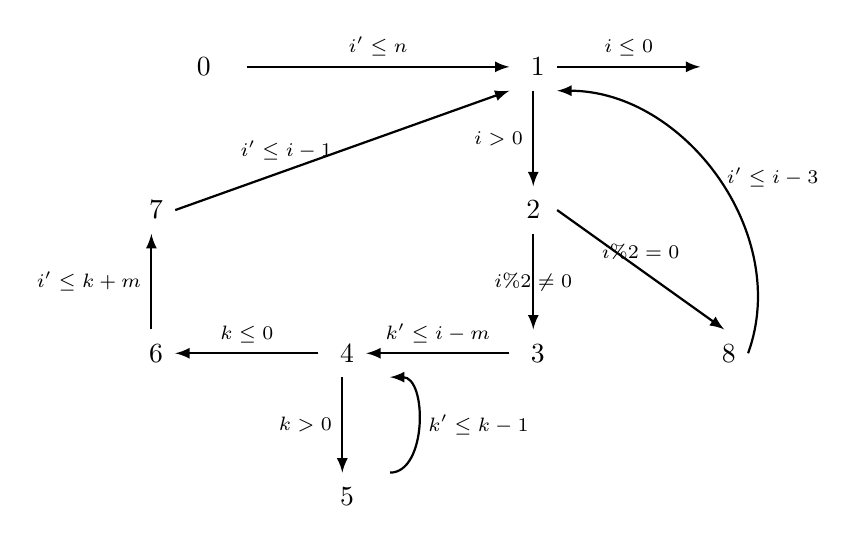
\begin{tikzpicture}[scale=\textwidth/20cm,samples=200]
  \draw[] (-7, 10) circle (0pt) node{{ $0$}};
  \draw[] (0, 10) circle (0pt) node{{ $1$}};
  \draw[] (0, 7) circle (0pt) node{\textbf{$2$}};
  \draw[] (0, 4) circle (0pt) node{{ $3$}};
  \draw[] (-4, 4) circle (0pt) node{{ $4$}};
  \draw[] (-8, 4) circle (0pt) node{{ $6$}};
  \draw[] (-4, 1) circle (0pt) node{{ $5$}};
  \draw[] (4, 4) circle (0pt) node{{ $8$}};
  \draw[] (-8, 7) circle (0pt) node{{ $7$}};
  % Counter Variables
  \draw[] (4.5, 10) circle (0pt) node {\textbf{$\lex$}};
  % \draw[] (6, 4) circle (0pt) node {{ $ex$}};
  %
  % Control Flow Edges:
  \draw[ thick, -latex] (-6, 10)    -- node [above] {\scriptsize $i' \leq n$}(-0.5, 10);
  \draw[ thick, -latex] (0, 9.5)    -- node [left] {\scriptsize $i > 0$} (0, 7.5) ;
  \draw[ thick, -latex] (0.5, 7)    -- node [above] {\scriptsize $ i \% 2 = 0 $}  (4, 4.5);
  \draw[ thick, -latex] (4.5, 4)    to  [out=70,in=0]   node [right] {\scriptsize $i' \leq i - 3$ }(0.5, 9.5);
  \draw[ thick, -latex]  (0, 6.5)   -- node  {\scriptsize $i \% 2 \neq 0$}  (0, 4.5) ;
  \draw[ thick, -latex]  (-0.5, 4)  -- node [above] {\scriptsize $k' \leq i - m$ }  (-3.5, 4) ;
  \draw[ thick, -latex]  (-4.5, 4)  -- node [above] {\scriptsize $k \leq 0$ }  (-7.5, 4);
  \draw[ thick, -latex] (0.5, 10)   -- node [above] {\scriptsize $i \leq 0$}  (3.5, 10);
  \draw[ thick, -latex] (-4, 3.5)   -- node [left] {\scriptsize $k > 0$}  (-4, 1.5);
  \draw[ thick, -latex] (-3, 1.5)   to  [out=0,in=0] node [right] {\scriptsize $k' \leq k- 1$}  (-3, 3.5);
  \draw[ thick, -latex] (-8, 4.5)   --  node [left] {\scriptsize $i' \leq k + m$ }(-8, 6.5);
  \draw[ thick, -latex] (-7.5, 7)  --  node [left] {\scriptsize $i' \leq i - 1$ }(-0.5, 9.5);
  % \draw[ thick, -latex] (6, 6.5)  -- node [right] {$\top$} (6, 4.5) ;
  \end{tikzpicture}
  \caption{}
    \end{centering}
    \end{subfigure}
\begin{subfigure}{.9\textwidth}    
\begin{centering}
  {\small
  $\tpath_0 = (0 \to 1)$
  \quad
  $\tpath_1 = (1 \to 2 \to 3 \to 4)$
  \quad
  $\tpath_2 = (4 \to 6 \to 7 \to 1)$
  \quad
  $\tpath_3 = (4 \to 5 \to 4)$
  \quad
  $\tpath_4 = (1 \to 2 \to 8 \to 1)$
  \quad
  $\tpath_5 = (1 \to \lex)$
  \\
  $
  \tpath_0 ; \rpchoose{ 1: \rprepeat(\tpath_1; 4:\rprepeat(\tpath_3); \tpath_2; \tpath_4), 
  1: \rprepeat(\tpath_4; \tpath_1; 4:\rprepeat(\tpath_3); \tpath_2) }; \tpath_5
  $
  }
  % \caption{}
    \end{centering}
    \end{subfigure}
  \caption{
  (a) The program of the two paths loop with a nested Loop in one path,
    (b) The corresponding \emph{Abstract Transition Graph}, $\absG(\kw{nestedOdd}(n, m))$. }
      \label{fig:relatedNestedWhileOdd-overview}
  \end{figure}
  }
  %
  \end{example}    
  
\footnotetext{We use the notation $(l_0 \to \cdots \to l_n)$ to denote a vertices sequence $(l_0, \cdots, l_n)$, and the constraint on each edge in each transition path are omitted for concise.}
% \todo{Shorten}
% \begin{itemize}
%   \item 
\textbf{Challenge I}
  In this example, given $n \geq m$,
the precise \emph{reachability-bound}s for control locations $4$ and $5$ are both $m \times \lfloor\frac{n}{m}\rfloor$,
for location $2$ and $3$ are $(m + 1) \times \lfloor\frac{n}{m}\rfloor + 1$, 
and $1$ for locations $0, 1$ and $\lex$. 
\highlight{Notice here, though within the same loop $L_2$, the bounds for locations $4$ and $5$ on the first branch, and $6$ on the second branch are different.}
\\
However, the state-of-art \emph{reachability-bound} analysis~\cite{GulwaniZ10}
gives the same \emph{reachability-bound}, $n + \lfloor\frac{n}{m}\rfloor$ for all the locations within the loop $L_2$, which is tight w.r.t. $L_2$'s iteration times but not for different locations inside $L_2$ without considering multiple paths.
Among works on program complexity, cost and loop bound analysis, \cite{GulwaniJK09} can also compute the tight bound on the loop iteration but not reachability-bound on each location path-sensitively.
Though we can use it as the \emph{reachability-bound} for location $1$ and $2$,
the \emph{reachability-bounds} for control locations $4, 5$ and $6$ are still unclear.

This motivates us the first key novelty -- the \emph{path reachability-bound} $\inoutB(\rprog, \tpath)$ for a loop free path $\tpath$ within a loop program $\rprog$ bounds the evaluation times of each loop free path instead of the entire multipath loop.
% \item 

\textbf{Challenge II}
  Then in line 8, $i$ is reset by $w$ and $w$ is reset by $j$ at line 5. So the
while $L_6$ is only executed in the first iteration of while loop $L_1$ and $L_3$.
% \\
The while loop $L_3$ at line 3 is executed only in 
the first $m - N$ iterations of the 
$L_1$ because $j$ is reset by $i$ in line 2.
% \\
So the total iterations of all the three loops is
$n + m^2 - m \times N$,
and the precise \emph{reachability-bound} for location $7$ inside the $L_6$ is $N$,
for locations $4, 5$ and $8$ between the $L_3$ and $L_6$ are $(n-N) \times (m - N)$,
and $n - N$ for locations $2$ and $9$.
% \\
\highlight{Notice here the \emph{reachability-bounds} for the locations inside the loop $L_6$ is 
the same as its innermost loop iteration bound.
% , as well as our \emph{path reachability-bound}.
However, for the locations between $L_3$ and $L_6$,
the \emph{reachability-bounds} are the multiplication of the inner and outer loop iteration bounds.}
\\
To the best of our knowledge, the loop bound analysis method in \cite{GulwaniJK09} can only give a loose bound $n + (m \times n) + N$ for the entire loop complexity, and 
the DC-based algorithm in \cite{SinnZV17} is able to
compute a better but still loose bound, $n + m^2 - m \times N$ on total iteration times.
None of them can give the precise \emph{reachability-bound} for every location in these nested loops,
which is non-trivial to compute even though knowing the loop bound.
% especially for the locations similar to $7$ in $\kw{threeNestedWhile}$.

\highlight{
This motivates use consider our second novel quantity --
the numbers of iterations of the outside loop $L_3$ and $L_1$ such that,
during these iterations, the loop $L_6$ is ``entered''. 
We call this the \emph{loop reachability} of the location within loop $L_6$ w.r.t the loops $L_3$ and $L_1$.
Then by multiplying the loop iteration bound of the $L_6$ with its \emph{loop reachability} times w.r.t the  $L_3$ and $L_1$, we can compute the precise
\emph{reachability-bounds} for location $7$.
}

\highlight{
This quantity isn't considered or computed in any of the previous works.
In the line of methods based on path refinement and loop summarization, the \emph{Progress Invariant} method in \cite{GulwaniJK09} is only able to compute
the
bound on iteration numbers
of the inner loop $L_6$ in each iteration of $L_3$ and $L_1$, which are both $N$.
So they have to over-approximate the reachability-bound for locations inside $L_6$ with the
overall program complexity by multiplication, i.e., $n + m^2 - m \times N$.
In the line of the \emph{amortized complexity analysis} through ranking function, the DC-based algorithm in \cite{SinnZV17}
is only able to
compute the combined loop bound and the local bound of each loop
separately as well.
% We are still unable to know the precise \emph{reachability-bound} for the locations in the innermost loop.
}
% \end{itemize}
With the two key novelties, our algorithm computes the reachability-bound for this example through the following steps.
% \paragraph{Main Steps of Path-sensitive Reachability-bound Analysis}
% \label{sec:static_rb}

\textbf{\emph{Step1: Program abstraction.}}
In Section~\ref{sec:progabs},
we first 
generate the \emph{Abstract Transition Graph} as in Figure~\ref{fig:relatedNestedWhileOdd-overview}(b).
Each edge $l \xrightarrow{dc} l'$ is an abstract transition $\absevent = (l, dc, l')$ annotated with a constraint $dc$ corresponding to the command of label $l$.

Then we abstract the program in the form of paths.
$$
\tpath_0 ; \rpchoose{ 1: \rprepeat(\tpath_1; 4:\rprepeat(\tpath_3); \tpath_2), 1:\rprepeat(\tpath_4) }; \tpath_5
$$
$;$ concatenates sequence of execution paths,
$\rprepeat(\tpath_3)$ represents looping on the path $\tpath_3$ and
$\rpchoose{ \ldots}$ represents the loop $L_1$ which contains two possible execution paths,
$\rprog_1 = \tpath_1; 4:\rprepeat(\tpath_3);\tpath_2$ and $\rprog_2 =\tpath_4$.

% \textbf{Step 2: Program Refinement}
\textbf{\emph{Step 2: Path interleaving refinement.}} 
Two execution paths are not simply iterating on themselves during the program execution,
they could interleave each other at certain iteration.
We summarize each execution path into conjunctions of transition relations.
\begin{equation}
    \begin{array}{l}
        \rprog_1 \models \phi_1 = \\
    \rprog_2 \models \phi_2 = 
    \end{array}
\end{equation}
  
In this sense, Algorithm~\ref{alg:prog-refine} in Section~\ref{sec:refine} computes the interleaving orders
by exhaustively checking the compositions of transition relations of different execution paths,
\begin{equation}
    \begin{array}{l}
        \rprog_1 ; \rprog_1 \models \exists i, k \st \phi_1 \circ \phi_1 = ... \implies \efalse\\
        \rprog_2 ; \rprog_2 \models \exists i, k \st \phi_2 \circ \phi_2 = ... \implies \efalse \\
        \rprog_2 ; \rprog_1 \models \exists i, k \st \phi_2 \circ \phi_1 = ...  \\
        \rprog_1 ; \rprog_2 \models \exists i, k \st \phi_1 \circ \phi_2 = ... 
    \end{array}
\end{equation}
Only two execution paths are feasible, so we identify two unique interleaving orders --
either $\rprog_1$ executes after one iteration of $\rprog_2$ or vice versa.
% Then, loop $L_1$ in the source program is generates new execution paths as follows,
\[
    \rprog^1 = \rprog_1 ; \rprog_2 = \tpath_1; 4:\rprepeat(\tpath_3); \tpath_2; \tpath_4
    \qquad
    \rprog^2 = \rprog_2 ; \rprog_1 = \tpath_4; \tpath_1; 4:\rprepeat(\tpath_3); \tpath_2
\]
% The second step in Section~\ref{sec:refine}
Then, the multiple-paths loop $L_1$ in the source program is refined
into multiple loops where each one can only iterate following the specified interleaving order.
% the interleaving of paths is explicit.
As in the bottom of Figure~\ref{fig:relatedNestedWhileOdd-overview}(c),
the program is transformed into 
\[
    \tpath_0 ; \rpchoose{ 1: \rprepeat(\tpath_1; 4:\rprepeat(\tpath_3); \tpath_2; \tpath_4), 
1: \rprepeat(\tpath_4; \tpath_1; 4:\rprepeat(\tpath_3); \tpath_2) }; \tpath_5
\]
In this refined program, 
each new execution path is equivalent to the execution of the original loop. 
% denoted as $\rprog_1^1$ and $\rprog_1^2$.

% \textbf{Step 3: Ranking Function Estimation}
\textbf{\emph{Step 3: ranking function estimation.}}
Algorithms in Section~\ref{sec:rank} identifies the ranking function for each transition edge, which is a symbol whose number of decreasing times can represent the number of execution of this edge.
For example for edge $4 \to 5$, its ranking function is $k$ and edges on $\tpath_1$, $\tpath_2$ and $\tpath_4$ all have $i$ as their ranking functions.

% \textbf{Step 4: Path-sensitive Reachability-bound Computation.}
\textbf{\emph{Step 4: local path reachability-bound.}}
For $\tpath_3$ in the program in Figure~\ref{fig:relatedNestedWhileOdd-overview}, we want to know how many times it is ``reached'' during the program execution.
From the refined program, $\tpath_3$ shows up in both newly generated execution paths $\rprog^1$ and $\rprog^2$  and nested in two level loops.
The algorithm in Section~\ref{sec:pathlocalrb} first
% computes a local \emph{path reachability-bound} for it w.r.t. its innermost loop $L_4$ by computing 
computes three abstract states for the ranking functions on $\tpath_3$ when first, second and last visiting during execution of $L_4$,
\begin{equation*}
    \rfinit(\rprog^1, \tpath_3, c) = \{k = n - m\} \quad
    \rfnext(\rprog^1, \tpath_3, c) = \{k = 1\} \quad
    \rffinal(\tpath_3, c) = \{ k = 0 \}.
\end{equation*}
Then  the maximal value of the following formula provides   
an upper bound on the number of execution times of $\tpath_3$ when executing only the innermost loop where $\tpath_3$ is nested. 
\[
    \max
    \left\{ 
        {\frac{a - b}{1}} 
        ~\vert~
        x = a \in \{k = n - m\}
        \land x = b \in \{ k = 0 \}
    \right\}  = n - m
\]
% The algorithm in Section~\ref{sec:pathlocalrb}
% computes $\outinB(4:\rprepeat(\tpath_3), \tpath_3, c) = n - m$ by computing
% the initial state, next state and final state of ranking functions on $\tpath_3$ during the execution of $\rprepeat(\tpath_3)$.

\textbf{\emph{Step 5: loop reachability-bound.}}
Previous step only provides the path reachability-bound for a simple transition path w.r.t. the innermost loop.
For nested loops, we need to compute the \emph{loop reachability-bound} for each simple transition path with respect to every level of the outer loop.
Since $\tpath_3$ is nested in two level loops, we compute its \emph{loop reachability-bound}
with respect to the outer loop $L_1$. 
It is expected to be $1$ because the inner loop $L_4$ is reached only in the first iteration of the outer loop $L_1$.
% , we aim to compute $1$ as the \emph{loop reachability-bound} of $\tpath_3$ w.r.t. $L_1$.
In the first refined execution path, $\rprog^1 = \rprepeat(\tpath_1; 4:\rprepeat(\tpath_3); \tpath_2; \tpath_4)$,
we compute three abstract states when visiting $L_4$ the first, second and last time during the execution of loop $\rprog^1$,
\begin{equation*}
\lpinit(\rprog^1, \tpath_3, c) = \max\{ n - m\} \quad
\lpnext(\rprog^1, \tpath_3, c) = \max\{n - m\} \quad
\rffinal(\tpath_3, c) = \{k = 0\}.
\end{equation*}
Then we compute \emph{loop reachability-bound} as the maximal value of the formula,
\[
    \max\limits_{x = a \in \{k = 0\}}
    \frac{\lpinit(\max\{n - m\} - a }{\max\{n - m\}} = 1
  \]
We also compute in the second refined execution path $\rprog_1^2$ the same number.
% $\outinB(4:\rprepeat(\tpath_3), \tpath, c) = n - m - 3$ and the same $\lpchB(\rprog_1^2, \tpath_3, c)$.
% So 

\textbf{\emph{Step 6: path reachability-bound.}}
For each simple transition path in every refined execution path where it shows up, we take the production of the \emph{loop reachability-bound}
and local \emph{path reachability-bound}.
For example for $\tpath_3$ in the first refined execution path 
$\rprepeat(\tpath_1; 4:\rprepeat(\tpath_3); \tpath_2; \tpath_4)$,
we compute $1 \times (n - m)$ and $1 \times (n - m - 3)$ in the second execution path.
Then we
take the maximal value over all refined execution order and
$\inoutB(\rprog, \tpath_3, c) = \max\{ 1 \times (n - m), 1 \times (n - m - 3) \} = n - m$.
This maximization operation does not produce over-approximation because there does not exist interleave
between the refined execution paths and each refined execution path is equivalent to the original loop, and each other as well.

\textbf{\emph{Step 7: reachability-bound.}}
Now for every program point $l$, we sum up the $\inoutB(\rprog, \tpath)$ over all $\tpath$ that contains $l$ and get $\psRB(l, c)$.
Since point $5$ only shows up on $\tpath_3$, we compute \highlight{$\psRB(5, c) = n - m$}.
The points $0$ and $\lex$ are not in any loop, so we have $\psRB(0, c) = \psRB(\lex, c) = 1$.
The points $3, 6, 7$ and $8$ which only show up once on $\tpath_2$ and $\tpath_4$ are all equal to $\lfloor\frac{m}{4}\rfloor$ the same as their $\inoutB$.
For the loop headers $1$ and $4$, we only count the $\tpath$ where they show up as a start-point.
So $\psRB(4, c) = \lfloor\frac{m}{4}\rfloor + n - m + 1$ and $\psRB(1,c) = 2 \times \lfloor\frac{m}{4}\rfloor + 1$ all as expected.


% % The second key idea combining two lines of works above is the \emph{loop reachability-bound}, $\lpchB(L:\rprog, \tpath)$.
% % For each transition path $\tpath$ w.r.t each of the loops $L:\rprog$ in which $\tpath$ is nested,
% % $\lpchB(L:\rprog, \tpath)$ bounds the iterations for
% % the outside loop, $L:\rprog$ w.r.t. the innermost loop where $\tpath$ is enclosed,
% % such that during these iterations of $L:\rprog$, the innermost loop is ``entered''. 
% % Then by multiplication and summing over these two bounds where each program control point shows up, we compute each point's the \emph{reachability-bound} path-sensitively.

% \paragraph{The path reachability-bound}, $\inoutB(\rprog, \tpath)$ is our first key novelty.
% It is a bound for a loop free path $\tpath$ within a loop program $\rprog$ bounds the evaluation times of each loop free path instead of the entire multipath loop.
% \input{examples/whileTwoCounters-overview}
% \footnotetext{We use the notation $(l_0 \to \cdots \to l_n)$ to denote a vertices sequence $(l_0, \cdots, l_n)$, and the constraint on each edge in each transition path are omitted for concise.}
% Figure~\ref{fig:whileTwoCounters-overview}(a) shows an example of a two paths loops
% with different \emph{reachability-bounds} on the control locations in different paths.
% This example is adopted from the example in~\cite{GulwaniZ10}, which
% is a skeleton code from the .Net base-class library.
% \\
% In this example, given $n \geq m$,
% the precise \emph{reachability-bound}s for control locations $4$ and $5$ are both $m \times \lfloor\frac{n}{m}\rfloor$,
% for location $2$ and $3$ are $(m + 1) \times \lfloor\frac{n}{m}\rfloor + 1$, 
% and $1$ for locations $0, 1$ and $\lex$. 
% \highlight{Notice here, though within the same loop $L_2$, the bounds for locations $4$ and $5$ on the first branch, and $6$ on the second branch are different.}
% \\
% However, the state-of-art \emph{reachability-bound} analysis~\cite{GulwaniZ10}
% gives the same \emph{reachability-bound}, $n + \lfloor\frac{n}{m}\rfloor$ for all the locations within the loop $L_2$, which is tight w.r.t. $L_2$'s iteration times but not for different locations inside $L_2$ without considering multiple paths.
% Among works on program complexity, cost and loop bound analysis, \cite{GulwaniJK09} can also compute the tight bound on the loop iteration but not reachability-bound on each location path-sensitively.
% Though we can use it as the \emph{reachability-bound} for location $1$ and $2$,
% the \emph{reachability-bounds} for control locations $4, 5$ and $6$ are still unclear.

% To compute the bounds for locations on different paths of a loop, we compute the \emph{path reachability-bound},
% which is the first key idea of this path-sensitive \emph{reachability-bound} analysis algorithm. This bound approximate the evaluation times of each loop free path instead of the entire multipath loop.
% \\
% This bound is computed based on the refined loop and using the estimated ranking function for every path, combines two lines of work introduced in Section~\ref{sec:intro}. It is benefited from the high accuracy of the path refinement and the ranking function estimation, but reduces the efficiency comparing to simply computing the ranking function.
% \\
% % Our algorithm combines the idea of \emph{difference constraint} based program complexity analysis method from \cite{SinnZV17}
% % and the control-flow refinement technique from~\cite{GulwaniJK09}.
% For this example, we first
% generate the abstract transition graph for the program using the difference constraints, such as Figure~\ref{fig:whileTwoCounters-overview}(b).
% Then it transforms every loop in $\kw{twoPathsWhile}$ by explicitly computing the interleaving between paths and
% %  using the control-flow refinement technique from~\cite{GulwaniJK09} and 
% generates a refined program $\rprog$ as
% \\
% % 
% % The refined program for program $\kw{twoPathsWhile}$ is
% % \[
%   $
%   \tpath_0 ; 
%   \rpchoose{2: \rprepeat_2(\rprepeat_1(\tpath_1); \tpath_2), 
%   2: \rprepeat_1(\tpath_1)}; \tpath_3.
%   $
% % \]
% \\
% Each $\tpath_i$ in this refined program is a \emph{simple transition path} we computed in a pre-procedure, which is loop free and not interleave with the other $\tpath_j, j \neq i$ as in Figure~\ref{fig:whileTwoCounters-overview}(c).
% % Every path will not interleave with the others. 
% Then we compute the \emph{path reachability-bound} for every $\tpath_i$,
% $\inoutB(\rprog, \tpath_i)$ during the execution of $\rprog$.
% % which is a bound on the reachability time of $\tpath$ during the execution of $\rprog$.
% The \emph{path reachability-bound}s for the four simple transition paths in this example are
% $\inoutB(\rprog, \tpath_1) = \max\{m, m \times \lfloor\frac{n}{m}\rfloor\}$,
% $\inoutB(\rprog, \tpath_2) = \lfloor\frac{n}{m}\rfloor$,
% and $\inoutB(\rprog, \tpath_0) = \inoutB(\rprog, \tpath_3) = 1$.
% % \\
% % Then we use this bounds
% % and another \emph{loop reachability-bound}
% % to compute the final \emph{reachability-bound} for each location.
% Since there isn't nested loop in this example, we simply sum up $\inoutB(\rprog, \tpath)$ over the $\tpath$ where a certain location shows up
% and as the \emph{reachability-bound} of this location.
% Then we get the precise \emph{reachability-bound} for every location in program $\kw{twoPathsWhile}$ as
% $\psRB(0) = \psRB(1) = \psRB(\lex) = 1$,
% $\psRB(4) = \psRB(5) = \max\{m, m \times \lfloor\frac{n}{m}\rfloor\}$,
% $\psRB(3) = \psRB(2) = \max\{m, m \times \lfloor\frac{n}{m}\rfloor\} + \lfloor\frac{n}{m}\rfloor + 1 $,
% and $\psRB(6) = \lfloor\frac{n}{m}\rfloor$.
% %

% However, when there exists nested loop, computing the \emph{reachability-bound} for each location encounters another challenge.
% The \emph{path reachability-bound} is precise for each path w.r.t. the innermost loop but not the outer nested loops.
% \paragraph*{Loop reachability-bound}, $\lpchB(L:\rprog, \tpath)$ is our second key idea combining two lines of works.
% It has high accuracy and efficiency by using the estimated ranking function based on the \emph{amortized complexity analysis} methodology over the refined loop paths.
% For each transition path $\tpath$ w.r.t each of the loops $L:\rprog$ in which $\tpath$ is nested,
% $\lpchB(L:\rprog, \tpath)$ 
% \highlight{is a bound on the iterations for
% the outside loop, $L:\rprog$ w.r.t. the innermost loop where $\tpath$ is enclosed,
% such that during these iterations of $L:\rprog$, the innermost loop is ``entered''. 
% This is distinguished from the traditional methods, which only estimate the bound on the inner loop's iteration number
% in one iteration of the outside loop.}

% Figure~\ref{fig:threeWhile-overview}(a) shows an example of the nested loops with related 
% iterators.
% This example is adopted from the example in~\cite{GulwaniJK09}, which is common in product code.
% \\
% In line 8, $i$ is reset by $w$ and $w$ is reset by $j$ at line 5. So the
% while $L_6$ is only executed in the first iteration of while loop $L_1$ and $L_3$.
% % \\
% The while loop $L_3$ at line 3 is executed only in 
% the first $m - N$ iterations of the 
% $L_1$ because $j$ is reset by $i$ in line 2.
% % \\
% So the total iterations of all the three loops is
% $n + m^2 - m \times N$,
% and the precise \emph{reachability-bound} for location $7$ inside the $L_6$ is $N$,
% for locations $4, 5$ and $8$ between the $L_3$ and $L_6$ are $(n-N) \times (m - N)$,
% and $n - N$ for locations $2$ and $9$.
% % \\
% \highlight{Notice here the \emph{reachability-bounds} for the locations inside the loop $L_6$ is 
% the same as its innermost loop iteration bound.
% % , as well as our \emph{path reachability-bound}.
% However, for the locations between $L_3$ and $L_6$,
% the \emph{reachability-bounds} are the multiplication of the inner and outer loop iteration bounds.}
% \\
% To the best of our knowledge, the loop bound analysis method in \cite{GulwaniJK09} can only give a loose bound $n + (m \times n) + N$ for the entire loop complexity, and 
% the DC-based algorithm in \cite{SinnZV17} is able to
% compute a better but still loose bound, $n + m^2 - m \times N$ on total iteration times.
% None of them can give the precise \emph{reachability-bound} for every location in these nested loops,
% which is non-trivial to compute even though knowing the loop bound,
% especially for the locations similar to $7$ in $\kw{threeNestedWhile}$.
% \\
% \highlight{
% In order to precisely compute how many times the location $7$ is reached, we need to know
% the numbers of iterations of the outside loop $L_3$ and $L_1$ such that,
% during these iterations, the loop $L_6$ is ``entered''. 
% We call this the \emph{loop reachability} of the location within loop $L_6$ w.r.t the loops $L_3$ and $L_1$.
% Then by multiplying the loop iteration bound of the $L_6$ with its \emph{loop reachability} times w.r.t the  $L_3$ and $L_1$, we can compute the precise
% \emph{reachability-bounds} for location $7$.
% }
% \\
% \highlight{
% This quantity isn't considered or computed in any of the previous works.
% In the line of methods based on path refinement and loop summarization, the \emph{Progress Invariant} method in \cite{GulwaniJK09} is only able to compute
% the
% bound on iteration numbers
% of the inner loop $L_6$ in each iteration of $L_3$ and $L_1$, which are both $N$.
% So they have to over-approximate the reachability-bound for locations inside $L_6$ with the
% overall program complexity by multiplication, i.e., $n + m^2 - m \times N$.
% In the line of the \emph{amortized complexity analysis} through ranking function, the DC-based algorithm in \cite{SinnZV17}
% is only able to
% compute the combined loop bound and the local bound of each loop
% separately as well.
% % We are still unable to know the precise \emph{reachability-bound} for the locations in the innermost loop.
% }
% \\
% Similar to the $\kw{twoPathsWhile}$ example, we also generate its abstract transition graph as well in Figure~\ref{fig:threeWhile-overview}(a),
% and compute its refined program,
% $\rprog = \tpath_0; 1: \rprepeat(\tpath_1;$ 
% $3: {\rprepeat(\tpath_2; 6 : {\rprepeat(\tpath_3)}; \tpath_4)}; \tpath_5);$ 
% $\tpath_6$,
% where the $\tpath_0, \ldots$ are shown in the middle part of Figure~\ref{fig:threeWhile-overview}(b).
% We use $\rprog_1$ and $\rprog_3$ denote the body of the loop $L_1$ and $L_3$ respectively as in the bottom part of Figure~\ref{fig:threeWhile-overview}(b).
% % to denote ${\rprepeat(\tpath_1; 3: {\rprepeat(\tpath_2; 6 : {\rprepeat(\tpath_3)}; \tpath_4)}; \tpath_5)}$
% % and $\rprog_3 = {\rprepeat(\tpath_2; 6 : {\rprepeat(\tpath_3)}; \tpath_4)}$
% In the first step, we still compute the \emph{path reachability-bound} for each $\tpath_i$ but only w.r.t. the innermost loop it is nested.
% Then differently from $\kw{twoPathsWhile}$,
% we compute \emph{loop reachability-bound} for each $\tpath_i$ w.r.t. each of its outer nested loops.
% For example, for $\tpath_3$ we compute
% $\lpchB(1: \rprog_1, \tpath_3) = 1$ and
% $\lpchB(3: \rprog_3, \tpath_3) = 1$.
% Both are tight because loop $L_6$ will only be entered once among all iterations of $L_1$ and $L_3$, and in all the rest iterations, the body of loop $L_6$ isn't executed at all.
% So $1$ as \emph{loop reachability-bound} of this path is tight w.r.t. both the loop $L_3$ and $L_1$.
% % In the same way, we also compute $\lpchB(3: \rprog_3, \tpath_3) = 1$ precisely.
% Then for each $\tpath_i$, the multiplication of its \emph{path reachability-bound} with all its \emph{loop reachability-bound}s is an accurate \emph{loop reachability-bound} for the locations on this path.
% By summing up the reachability-bound of the path where each location shows up,
% % as its \emph{reachability-bound} as before.
% % and multiply this result by all its \emph{loop reachability-bound}s.
% % In this way, 
% we compute $N$ as the \emph{reachability-bound} of location $7$, which is tight.
%     %
    \begin{figure}
    \centering
    %
    \begin{subfigure}{.45\textwidth}
        $
        \begin{array}{l}
            N < m < n\\
            \kw{threeNestedWhile}(n, m, N) \triangleq \\
            \clabel{ \assign{i}{0} }^{0} ; \\
                L_1: \ewhile ~ \clabel{i < n}^{1} ~ \edo ~ \\
                \quad \Big(
                 \highlight{\clabel{\assign{j}{0}}^{2}} ;\\
                 L_3:  \quad \ewhile ~ \clabel{j < m}^{3} ~ \edo ~ \\
                \quad \quad \Big( \clabel{\assign{j}{j+1}}^{4};\\
                  \quad \quad \highlight{\clabel{\assign{w}{i}}^{5}};\\
                  L_6:  \quad \quad \ewhile ~ \clabel{w < N}^{6} ~ \edo ~ \\
                  \quad \quad \quad \Big( \clabel{\assign{w}{w + 1}}^{7}
                      \Big); \\
                      \quad \quad \clabel{\assign{i}{w}}^{8}
                      \Big); \\
                      \quad \clabel{\assign{i}{i+1}}^{9}
                  \Big)
            \end{array}
            $
    \caption{}
        \end{subfigure}
    \begin{subfigure}{.48\textwidth}
        \begin{centering}
            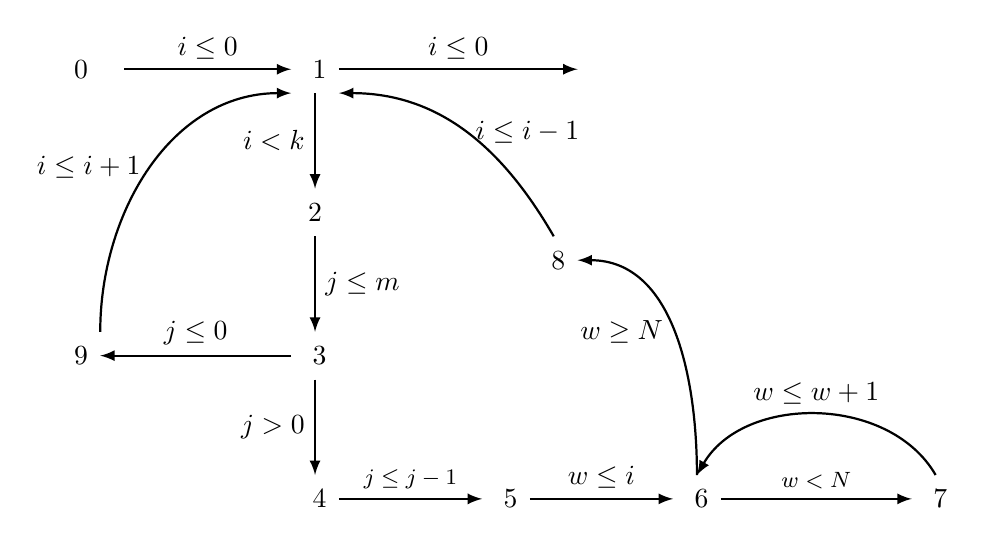
\begin{tikzpicture}[scale=\textwidth/20cm,samples=200]
                \draw[] (-5, 10) circle (0pt) node{{ $0$}};
                \draw[] (0, 10) circle (0pt) node{{ $1$}};
                \draw[] (6, 10) circle (0pt) node {{$\lex$}};
                \draw[] (0, 7) circle (0pt) node{{$2$}};
                \draw[] (0, 4) circle (0pt) node{{ $3$}};
                \draw[] (-5, 4) circle (0pt) node{{ $9$}};
                \draw[] (0, 1) circle (0pt) node{{ $4$}};
                \draw[] (4, 1) circle (0pt) node{{ $5$}};
                \draw[] (8, 1) circle (0pt) node{{ $6$}};
                \draw[] (13, 1) circle (0pt) node{{ $7$}};
                \draw[] (5, 6) circle (0pt) node{{ $8$}};
                % Counter Variables
                %
                % Control Flow Edges:
                \draw[ thick, -latex] (-4, 10)  -- node [above] {$i \leq 0$}(-0.5, 10);
                \draw[ thick, -latex] (0, 9.5)  -- node [left] {$i < k$} (0, 7.5) ;
                \draw[ thick, -latex] (0, 6.5)  -- node [right] {$j \leq m$} (0, 4.5) ;
                \draw[ thick, -latex] (0, 3.5)  -- node [left] {$j > 0$} (0, 1.5) ;
                \draw[ thick, -latex] (-0.5, 4)  -- node [above] {$j \leq 0$} (-4.5, 4) ;
                \draw[ thick, -latex] (-4.5, 4.5)  to  [out=90,in=180]  node [left] {$i \leq i + 1$ }(-0.5, 9.5);
                \draw[ thick, -latex] (0.5, 10)  -- node [above] {$i \leq 0$}  (5.5, 10);
                \draw[ thick, -latex] (0.5, 1)  -- node [above] {{\footnotesize $j \leq j - 1$}}  (3.5, 1);
                \draw[ thick, -latex] (4.5, 1)  -- node [above] {$w \leq i$}  (7.5, 1);
                \draw[ thick, -latex] (8.5, 1)  -- node [above] {{\footnotesize $w < N$}}  (12.5, 1);
                \draw[ thick, -latex] (8, 1.5)  to [out=90,in=0] node [left] {{$w \geq N$}}  (5.5, 6);
                \draw[ thick, -latex] (13, 1.5)  to  [out=120,in=60] node [above] {$w \leq w + 1$}  (8, 1.5);
                \draw[ thick, -latex] (5, 6.5)  to  [out=120,in=0]  node [right] {$i \leq i - 1$ }(0.5, 9.5);
                \end{tikzpicture}
%     \caption{}
%     \end{centering}
%     \end{subfigure}
% \begin{subfigure}{.2\textwidth}    
% \begin{centering}
    {\small
$
    \begin{array}{ll}
        \tpath_0 = (0 \to 1)
        &
        \tpath_4 = (6 \to 8 \to 3)
        \\        
        \tpath_1 = (1 \to 2 \to 3)
        &
        \tpath_5 = (3 \to 9 \to 1)
        \\
        \tpath_2 = (3 \to 4 \to 5 \to 6)
        &
        \tpath_6 = (1 \to \lex)
        \\
        \tpath_3 = (6 \to 7 \to 6)
    \end{array}
$
$
    \begin{array}{l}
        \rprog_1 = {\rprepeat(\tpath_1; 3: {\rprepeat(\tpath_2; 6 : {\rprepeat(\tpath_3)}; \tpath_4)}; \tpath_5)}
        \\
        \rprog_3 = {\rprepeat(\tpath_2; 6 : {\rprepeat(\tpath_3)}; \tpath_4)}
    \end{array}
$
}
\caption{}
\end{centering}
\end{subfigure}
    \caption{
    (a) An example of three nested loops with related iterator variables.
    (b) The abstract transition graph, simple transition paths and loop body.}
        \label{fig:threeWhile-overview}
    \end{figure}
